% ****** Start of file apssamp.tex ******
%
%   This file is part of the APS files in the REVTeX 4.2 distribution.
%   Version 4.2a of REVTeX, December 2014
%
%   Copyright (c) 2014 The American Physical Society.
%
%   See the REVTeX 4 README file for restrictions and more information.
%
% TeX'ing this file requires that you have AMS-LaTeX 2.0 installed
% as well as the rest of the prerequisites for REVTeX 4.2
%
% See the REVTeX 4 README file
% It also requires running BibTeX. The commands are as follows:
%
%  1)  latex apssamp.tex
%  2)  bibtex apssamp
%  3)  latex apssamp.tex
%  4)  latex apssamp.tex
%
\documentclass[%
 reprint,
superscriptaddress,
%groupedaddress,
%unsortedaddress,
%runinaddress,
%frontmatterverbose, 
%preprint,
%preprintnumbers,
nofootinbib,
%nobibnotes,
%bibnotes,
 amsmath,amssymb,
 aps,
%prd,
prl,
%rmp,
%prstab,
%prstper,
%floatfix,
]{revtex4-2}

\usepackage{graphicx}% Include figure files
\usepackage{dcolumn}% Align table columns on decimal point
\usepackage{bm}% bold math
\usepackage{lipsum}% http://ctan.org/pkg/lipsum
\usepackage{xfrac}

\usepackage{hyperref}% add hypertext capabilities
\usepackage{amssymb}
%\usepackage[mathlines]{lineno}% Enable numbering of text and display math
%\linenumbers\relax % Commence numbering lines

%\usepackage[showframe,%Uncomment any one of the following lines to test 
%%scale=0.7, marginratio={1:1, 2:3}, ignoreall,% default settings
%%text={7in,10in},centering,
%%margin=1.5in,
%%total={6.5in,8.75in}, top=1.2in, left=0.9in, includefoot,
%%height=10in,a5paper,hmargin={3cm,0.8in},
%]{geometry}

\begin{document}

%\preprint{APS/123-QED}

\title{Quartz fluorescence backgrounds in rare-event searches}% Force line breaks with \\
%\thanks{A footnote to the article title}%



\author{P. Sorensen}\email{pfsorensen@lbl.gov}
\affiliation{Lawrence Berkeley National Laboratory, 1 Cyclotron Rd, Berkeley, CA 94720, USA}
\author{R. Gibbons}%\email{rgibbons@berkeley.edu}
\affiliation{Lawrence Berkeley National Laboratory, 1 Cyclotron Rd, Berkeley, CA 94720, USA}
\affiliation{University of California, Berkeley, Department of Physics, Berkeley, CA 94720, USA}


\date{\today}% It is always \today, today,
             %  but any date may be explicitly specified

\begin{abstract}
It has been known for almost a decade that delayed photon noise with a power law time profile follows scintillation pulses in liquid xenon particle physics detectors. In the past two years, this noise has become a dominant background for low-threshold dark matter searches aimed at O(10)~GeV dark matter particle masses, as well as measurements of coherent neutrino-nucleus scattering of 8B solar neutrinos. We show that the dominant component of this delayed photon noise is due to UV-induced fluorescence of quartz photosensor windows.
\end{abstract}

%\keywords{Suggested keywords}%Use showkeys class option if keyword
                              %display desired
\maketitle

%\tableofcontents

%Main points
%\begin{enumerate}
%    \item Delayed photon emission is caused by fluorescence of X
%    \item Fluorescence is not affected by the amount of impurities in the detector
%    \item Fluorescence is affected by the size of the progenitor signal, and can be induced by introducing light
%    \item Delayed electron emission is dependent on the amount of impurities in the xenon
%    \item Delayed electron emission can be induced by introducing more fluorescence
%\end{enumerate}

%\section{\label{sec:level1}Introduction}

Astrophysical observations and cosmological data indicate the existence of non-luminous, non-baryonic massive dark matter~\cite{Planck:2018vyg,Sofue:2000jx}. 
A favored candidate for this dark matter has been a hypothetical class of beyond-the-Standard-Model particles called Weakly Interacting Massive Particles (WIMPs) with typical masses in the range of 100 GeV/c\textsuperscript{2}~\cite{Schumann:2019eaa}. The most sensitive experiments searching for these particles use liquid xenon as a scattering target~\cite{LZ:2024zvo,XENON:2025vwd,PandaX-4T:2021bab}.

It has been known for more than a decade that ionizing events due to particle interactions in dual-phase liquid xenon Time-Projection Chambers (TPCs) are followed by a trickle of single electrons \cite{XENON10:2011prx} extending in time for tens to hundreds of milliseconds after the originating event. This delayed electron noise presents a fatal background for sub-GeV-mass dark matter searches in this class of detector \cite{Essig:2012yx}. It was later found to be accompanied by delayed photon noise, and both were initially incorrectly characterized by an exponential decay constant of a few milliseconds \cite{Sorensen:2017kpl}. Subsequent work \cite{LUX:2020vbj} showed that the electron and the photon afterglow follow a power law $d_p(t) = \alpha\bar{a}t^b$ with $\alpha$ proportional to the magnitude $\bar{a}$ of the originating 175~nm UV photon pulse, $b=-1.1$ for the electron noise and $b=-0.5$ for the photon noise. Recent investigation of the delayed photon noise in LZ found $b=-1.3$ \cite{Anderson-thesis}. 
%Further investigation affirmed this characterization of the delayed electron noise \cite{XENON:2021qze,Kopec:2021ccm}.  

%Coupled with an O(10)~Hz event rate, the delayed backgrounds are always present. Figure 2 from Ref. \cite{LUX:2020vbj} and Fig. 1 from Ref. \cite{XENON:2021qze} give a particularly clear view of the severity of the problem.
\begin{figure}[hb]
    \centering
    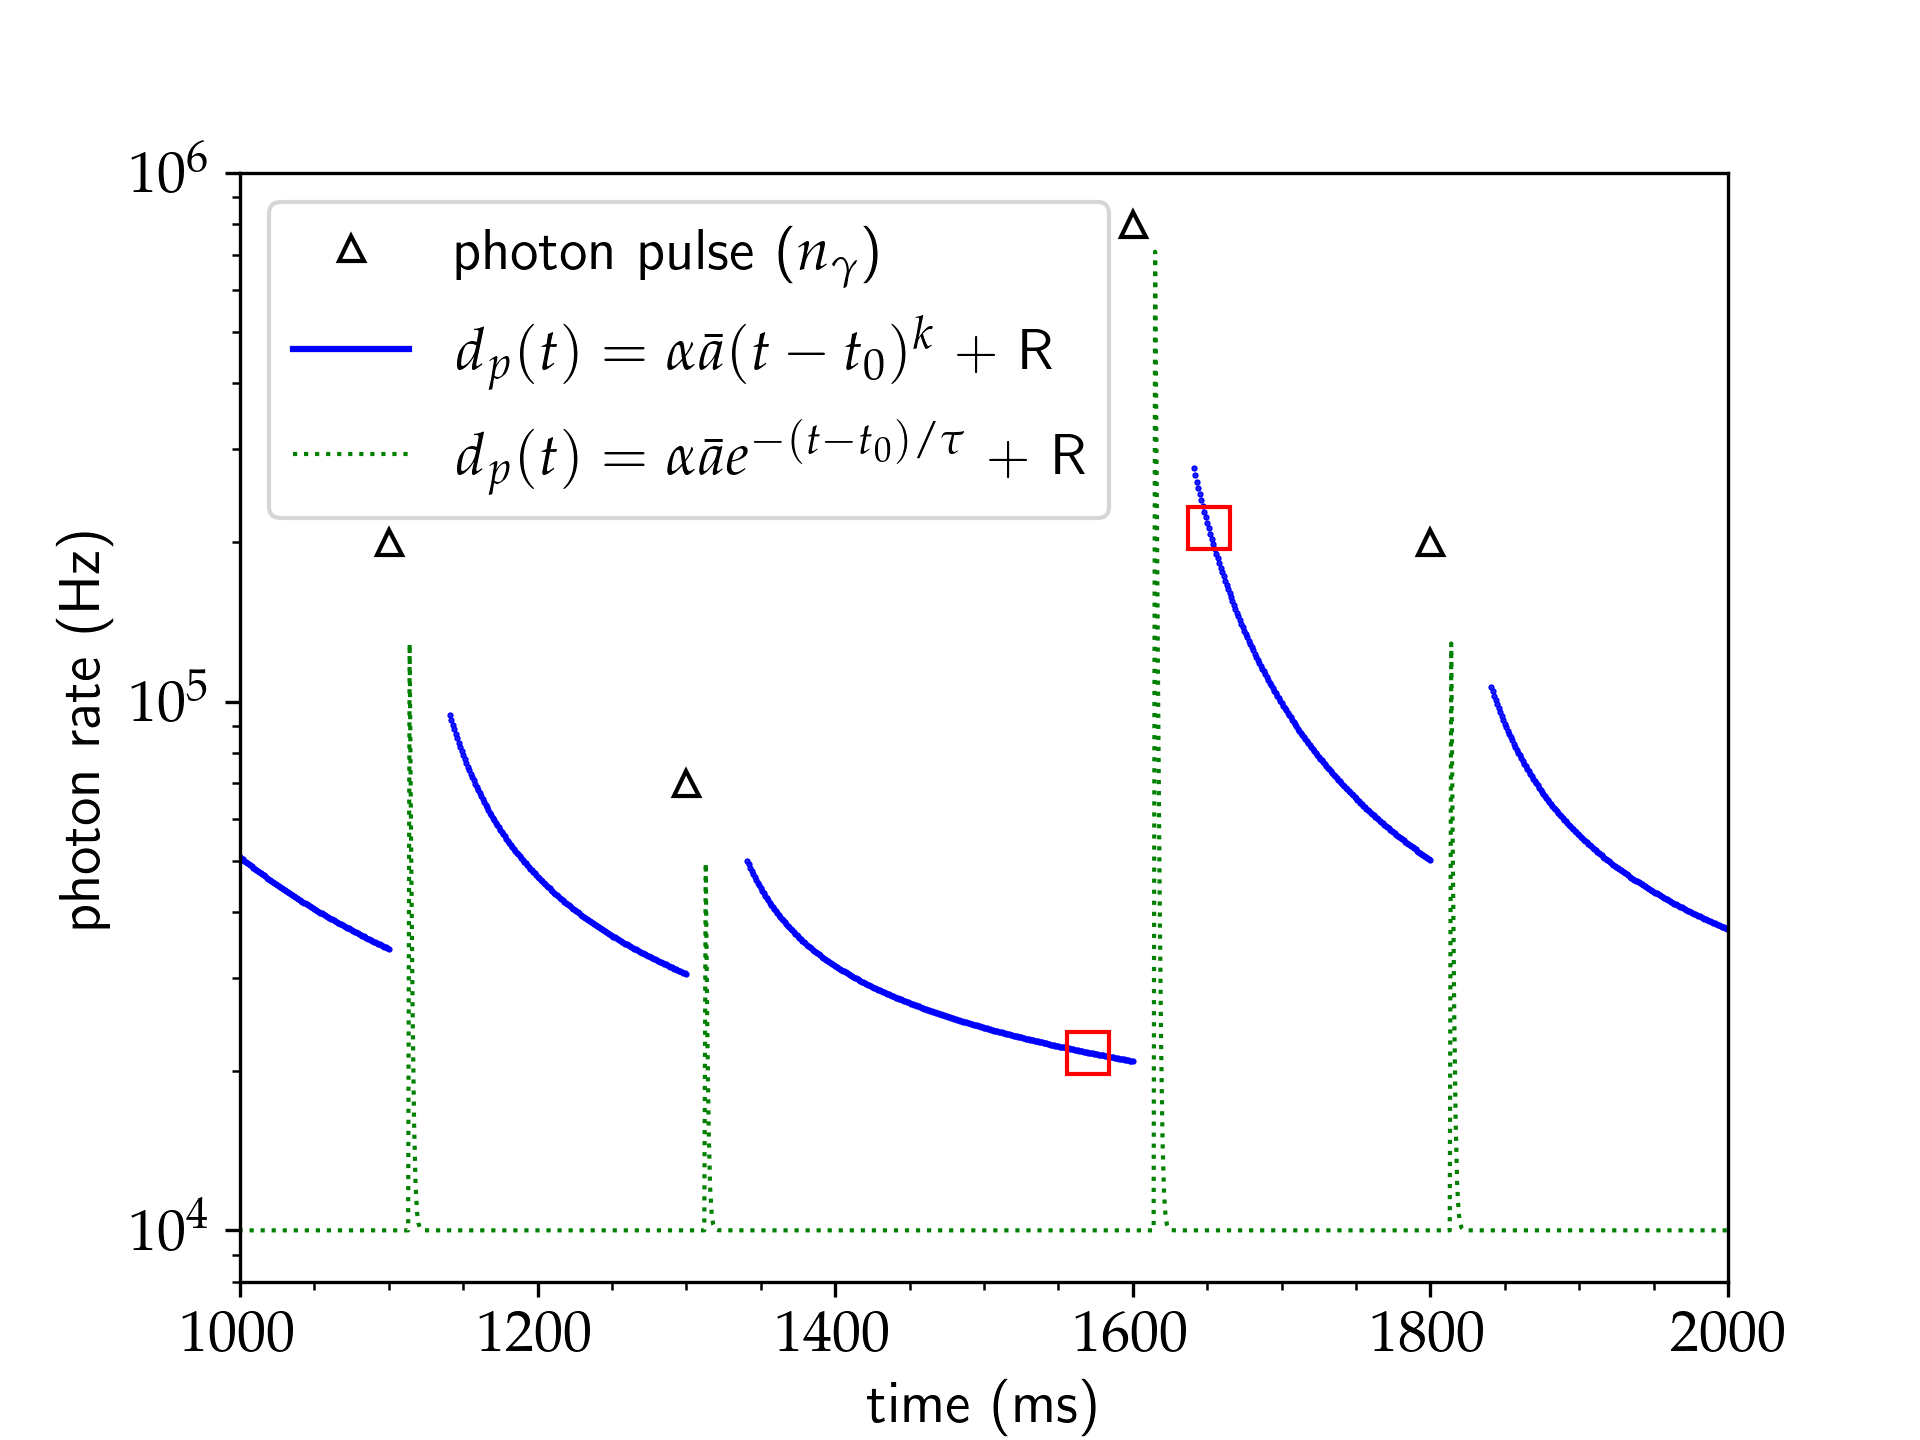
\includegraphics[width=0.49\textwidth]{figs.000.png}
    \caption{The delayed photon problem as exemplified by LZ, reproduced from \cite{Anderson-thesis}.}
   \label{fig:photon-rate}
\end{figure}

It is only recently that accidental coincidence (AC) backgrounds $-$ two more more random photon counts piling up in time to fake a small xenon scintillation signal $-$ have become dominant in searches for low-mass dark matter and observation of $^8$B solar neutrinos \cite{PandaX:2022aac,XENON:2024ijk}. This is a reflection of the incredibly low backgrounds these experiments have achieved. But it is somewhat striking nonetheless, because in the planning phases of these experiments, accidental coincidence backgrounds were either not mentioned \cite{XENON:2024wpa}, or were dismissed \cite{Mount:2017qzi} as sub-dominant. Typical measured thermal dark count rates are about 40~Hz for the 3" $\varnothing$ PMT used in these experiments. The total photon rate for a detector instrumented with 500 such PMTs is therefore about 20~kHz, which for a steady-state background rate would give an accidental 2-fold photon coincidence pileup rate of about 2~Hz (check this). While some AC backgrounds result from the dark count rate, delayed photon noise can easily increase the total photon rate up by a factor $\times 10$ or more, and is thus a serious problem. This is exemplified in Fig. \ref{fig:photon-rate}. Note that particle interaction events in this calss of TPCs consist of a primary scintillation pulse of UV photons (S1), followed by electron drift, electron emission into the vapor, and then electron-induced proportional scintillation pulse of UV photons (S2) up to about a millisecond later. The amplitude of a typical S2 pulse is a detector-dependent $\bar{a}\sim10^6$ for a 1 MeV electron interaction.
%And reasonably so: the Poisson probability for pileup based on measured thermal dark count rates of $<1$~Hz/cm$^2$ \cite{Baudis:2013xva} in the photomultiplier tubes (PMTs) indeed should be sub-dominant. However, the observed photon rate is significantly in excess of this value.

\begin{figure*}[ht]
    \centering
    \includegraphics[width=0.49\textwidth]{figs.001.png}
    \includegraphics[width=0.49\textwidth]{figs.002.png}
    \caption{Measurements of the delayed photon noise count rate per 0.1~ms, following a pulse $\bar{a}$ of UV photons. The experimental configuration is indicated (inset). \textbf{(left)} With xenon in the active region, replicating the problem facing dark matter search experiments such as LZ, XENON and PandaX. \textbf{(right)} With vacuum in the active region. The spectrum of $d_p(t)$ shows the range of expected delayed noise for a range of xenon scintillation pulse sizes. }
   \label{fig:xe}
\end{figure*}

A fundamental question has remained: what is the origin of the delayed photons? We have investigated this issue with a 5~cm $\varnothing$ cylindrical testbed at LBL and conclude that the majority of the delayed photon noise is due to fluorescence of quartz\footnote{optical grade SiO$_2$ is often referred to interchangeably in technical literature as fused silica, synthetic silica or quartz} photosensor windows, following exposure to the UV photons from xenon scintillation.

%\emph{Experiment$-$} 
We initially\cite{Sorensen:2024idm} studied the delayed photon noise with the testbed operated as a TPC, i.e. with S1 and S2 pulses, in the style of the dark matter search experiments \cite{PandaX:2022aac,XENON:2024ijk}. We subsequently realized that a similar magnitude and time profile of delayed photon noise was also observed following the primary scintillation pulse (S1). The present work is therefore restricted to this simpler case using only S1 pulses, with no applied electric field and no S2 pulse. 

So that we could accurately count $\mathcal{O}(10)$~ns wide delayed single photon signals over a period of milliseconds following each progenitor pulse, we employed a cascade trigger: for each pulse, we recorded the 100~$\mu$s window containing that event, and also three additional 100~$\mu$s windows delayed by several hundred microseconds each. This allowed us to methodically sample the photons at later times, without loss of fidelity and within the capabilities of the data acquisition. The trigger time was set at 10~$\mu$s in the progenitor pulse window, which allowed an additional data point to be acquired from the last 50~$\mu$s of the trigger window. 



%Measurements of the average xenon scintillation signals and their delayed photons $d_p(t) = (a_0/xxxx) t^{-1.1}$ are shown in Fig. 1. 
The average response of many such measurements is shown in Fig. \ref{fig:xe} (left). Delayed photon counts are normalized to $100~\mu$s bin width, such that the delayed photon rate in Hertz is a factor $\times10^4$ larger. The initiating pulse width was $<1~\mu$s, and for the PMT data shown here consisted of $\bar{a}=2871$~ prompt scintillation photons detected. The scintillation decay times are $\tau=4$~ns and $\tau=27$~ns \cite{}, so they are completely exhausted within a few hundred nanoseconds. The magnitude and time profile of the delayed photon noise is fit by $d_p(t) = (\bar{a}/6086) t^{-1.30}$, and for the S13371 SiPM is $d_p(t) = (\bar{a}/2478) t^{-1.04}$. We observe that for PMT signals greater than a few hundred photons, PMT after-pulsing \cite{} systematically increases the photon counts in the $50-100~\mu$s bin, so this data point is excluded from the fit. 
%We observe a non-linearity in the amplitude and time profile of $d_p(t)$, as a function of the size of the initial UV pulse. This is discussed briefly in the appendix.

A 2D schematic of the cylindrical experimental configuration is shown in Fig. \ref{fig:xe} (inset), indicating the single PMT and the array of four four-channel Hamamatsu S13371 silicon photomultipliers (SiPM) viewing the active region filled with liquid xenon. Walls were constructed of PTFE, with several 1~mm~$\varnothing$ radial holes (not shown) allowing xenon to flow into and out of the active region. A single high-transparency mesh grid  bifurcated the region, and a $^{210}$Po alpha particle source plated in the center of the mesh caused xenon scintillation pulses at a rate of about 10~Hz. We verified (by removal) that the mesh is unrelated to the presence of the delayed photon noise. The testbed was maintained at a constant temperature $T=-99\pm1$~C, with a systematic (calibration) uncertainty of about 1~C. 

In order to test the hypothesis that fluorescence of the quartz window causes delayed photons, we made the same series of measurements with vacuum in the active region instead of liquid xenon.  The temperature was again maintained at $T=-99\pm1$~C. Gaseous xenon was used to thermalize the entire testbed for a period of several days, after which it was recovered and the active region was evacuated to a pressure of $1\times10^{-6}$~mBar. This low pressure was maintained by constant pumping during the experiment. Cherenkov photons from radioactive decays and Compton scatters in the window of the PMT were used as a source of UV photon pulses. We estimate the PMT might detect approximately 300 Cherenkov photons from a 1~MeV beta in glass. The total path length of such a particle is  expected to be 1.8~mm, while the PMT window is about 2~mm thick. The Cherenkov signal decays more quickly than xenon scintillation and has no intrinsic afterglow. It also has a broader spectrum than the 175~nm xenon scintillation, rising sharply at shorter wavelengths. Quartz transparency cuts off at about $\lambda=160$~nm.
%\footnote{Inexpensive, easily-deployable sources of UV photons in the absence of xenon scintillation was non-trivial: LEDs with $\lambda<235$~nm are not readily available, and in any case all LEDs we tested feature their own intrinsic afterglow.}

The magnitude and time profile of delayed photon noise observed from Cherenkov pulses in the absence of xenon are shown in Fig. \ref{fig:xe} (right). Due to the small average progenitor pulse $\bar{a}$, the response of the S13371 SiPM sensors was barely above the background photon count rate and is not shown. We also note that the quartz window on these sensors was thinner, specified at $0.5$~mm. We therefore could not easily use them as a source of Cherenkov photons. 

We wish to compare these data with the delayed photon noise measured following xenon scintillation pulses, but observe that for small signals, $d_p(t)$ depends on the number of photons observed by the S13371. We interpret this as a systematic effect on small signals, rather than a real, physical effect. To indicate this uncertainty, we show a spectrum of $d_p(t)$ curves, ranging from $\bar{a}\sim1000$~photons recorded in the S13371 (red)  $\bar{a}\sim3000$~photons observed in the S13371 array. 

%The spectrum of power laws shown were obtained from not a fit, but instead is the same $d_p(t)=(a_0/8000)t^{-1.1}$ as previously shown in Fig. 1, where now $a_0=334$ is the average number of detected Cherenkov trigger photons. The delayed noise triggered by Cherenkov photons appears to favor a slightly shallower power law exponent than $b\sim-1.1$. This may be due to the wavelength difference between the xenon photon source (175~nm) and the Cherenkov photon source (broad spectrum above 160~nm). 

%We do not consider the difference to be particularly significant for the purposes of rare-event search particle detection: the important point is that majority (if not all) of the power-law delayed photon noise appears to result from UV-catalyzed fluorescence of the SiO$_2$ windows of the photosensors.

%In spite of this systematic uncertainty, we see that the range of expectations is consistent with the measured SiO$_2$ fluorescence.

These measurements confirm that quartz is a source of fluorescence, and despite the systematic uncertainty just discussed, suggest that it may be the dominant source of delayed photon noise in detectors with liquid xenon as the active target medium. 

In order to conclusively identify quartz fluorescence as the primary cause of delayed photon noise in liquid xenon TPCs, we adapted the experimental configuration as shown in Fig. \ref{fig:no-window}: the active region was divided with a piece of aluminum, in order to optically isolate the upper and lower halves. The PMT was replaced with an array of four, windowless Hamamatsu S13370 SiPM. Of the four sensors, two had excessive leakage current and so were not biased. Of the remaining two, one showed lower dark counts and so we only report data from that single sensor. Given this, only a single channel of the 32 S13371 sensors was used to compare. The active region was completely filled with liquid xenon, and a flow-through $^{220}$Rn alpha particle source was used to provide xenon scintillation pulses. Because of the optical isolation, triggering on a pulse from the S13371 sensor was accompanied by random (mostly zero) photon counts in the S13370 sensor, and vice versa. 

The data were acquired separately and are shown together in Fig. \ref{fig:no-window}. The S13371 sensor shows $d_p(t) = (\bar{a}/5932)t^{-1.29}$. The S13371 random photon background is about 0.03 counts/0.1 ms and is not shown. In the absence of a window, a smaller, residual component to the delayed photon noise given by $d_p(t) = (\bar{a}/2536) t^{-0.16}$. The fluorescence is reduced by a factor $\times8$ in the $50-100~\mu$s bin. We attribute the difference in power law exponent to differences in impurities in the quartz windows of different devices. This residual component could be due to fluorescence of the silicon sensor, the ceramic package of the sensor, the PTFE or its impurities, impurities within the xenon or perhaps the xenon itself. We did previously explore varying states of degraded xenon purity and saw no significant difference in the measured $d_p(t)$. However, those investigations were made with S13371 sensors, so the quartz fluorescence may have obscured subtler effects.

\begin{figure}[ht]
    \centering
    \includegraphics[width=0.49\textwidth]{figs.003.png}
    \caption{Delayed photon noise measured in two symmetric, optically isolated regions, one with an quartz window and one without.}
   \label{fig:no-window}
\end{figure}

We have shown for the first time that the dominant component of delayed photon noise in liquid xenon particle physics detectors results from fluorescence of quartz windows in the photosensors. Glass is known to fluoresce due to point defects such as color centers, and because of impurities\cite{Jedamzik:2017,Corujo:2022}.  The fluorescence is often referred to as phosphorescence when the lifetime extends into the ms regime \cite{Jedamzik:2017} (as in the present case). A very high purity quartz called VIOSIL manufactured by Shin-Etsu \cite{Shinetsu} appears to have no measured fluorescence, in contrast to fused quartz. The windows used in the Hamamatsu sensors are specified as ``synthetic silica.'' We are not aware of any other measurements of the time dependence of quartz glass fluorescence.

 This information comes too late to help the current generation of leading dark matter search instruments, but it could be critical to the design choices of future experiments, such as the proposed XLZD experiment \cite{Aalbers:2022dzr}. For example, if PMTs are to continue to be used as photosensors, new R\&D would be needed to minimize the UV-induced fluorescence from window materials such as quartz, MgF, and others. Alternatively, silicon photomultipliers do not strictly need a window at all, other than to protect the sensitive silicon detection and gain structures. Silicon-based sensors do have other challenges, such as higher dark count rates even for optimized devices \cite{Sakamoto:2023ond} as well as the the so-called flashlight effect \cite{Gibbons:2023iux}. At the least, they should be useful for further investigation of the origins of the residual component of delayed photon noise, seen in Fig. \ref{fig:no-window}.





% *** more comment on effect to dark matter search outcomes



\begin{acknowledgments}
We thank Prof. Shingo Kazama for pointing out the Shin-Etsu quartz literature.

\end{acknowledgments}

\bibliography{phtrain}% Produces the bibliography via BibTeX.


\end{document}
%
